\documentclass[a4paper,12pt]{article}

\usepackage{cmap}          % поиск в PDF
\usepackage{mathtext}         % русские буквы в формулах
\usepackage[T2A]{fontenc}      % кодировка
\usepackage[utf8]{inputenc}      % кодировка исходного текста
\usepackage[english,russian]{babel}  % локализация и переносы
\usepackage[left=2cm,right=2cm,top=2cm,bottom=2cm]{geometry}
\usepackage{amsfonts,amssymb,amsthm,mathtools} % AMS
\usepackage{amsmath}
\usepackage{icomma} % "Умная" запятая: $0,2$ --- число, $0, 2$
\usepackage{graphicx}
\usepackage{wrapfig} % картинка в тектсе
\usepackage{caption} % убирается номер у подписей caption*{}
\usepackage{csquotes} % цитаты
\usepackage{multirow} % для жестких таблиц
\usepackage{hhline}
\usepackage{indentfirst} % абзацный отступ после section
\usepackage{epigraph} % эпиграф
\usepackage{tikz}
\usepackage{pgfplots}
\usepackage[export]{adjustbox}
\usepackage{tabularx}
\usepackage{float}
\usepackage{longtable}


\graphicspath{{pictures/}}
\begin{document}
	\pagenumbering{gobble}
	\pagenumbering{arabic}
	
	\title{\textbf{Получение и измерение вакуума. (2.3.1)}}
	\author{Зайнуллин Амир Б05-206}

	\maketitle

    \section{Аннотация}

	\textbf{Цель работы:} 1) измерение объёмов форвакуумной и высоковакуумной частей установки; 2) определение скорости откачки системы в стационарном режиме, а также по ухудшению и по улучшению вакуума.

    \textbf{В работе используются:} вакуумная установка с манометрами: масляным, термопарным и ионизационным.
	
    В данной работе изучаются традиционные методы откачки механическим насосом до давления $10^{-2}$ торр и диффузионым масляным насосом до давления $10^{-5}$ торр, а также методы измерения вакуума в этом диапазоне.



    \section{Теоретические сведения}

    \subsection*{Процесс откачки}
	Производительность насоса определяется скоростью откачки $W$ (л/с): $W$ — это объем газа, удаляемого из сосуда при данном давлении за единицу времени.

    Рассмотрим обычную схему откачки. Обозначим через $Q_d$ количество газа, десорбирующегося с поверхности откачиваемого объема в единицу времени, через $Q_i$ — количество газа, проникающего в единицу времени в этот объем извне — через течи. Будем считать, что насос обладает скоростью откачки $W$ и в то же время сам является источником газа; пусть $Q_n$ — поток газа, поступающего из насоса назад в откачиваемую систему. Будем измерять количество газа $Q_d$, $Q_i$ и $Q_n$. Основное уравнение, описывающее процесс откачки, имеет вид

    \begin{equation}
    	-VdP=(PW-Q_d-Q_n-Q_i)dt.
    \end{equation}

    Левая часть этого уравнения равна убыли газа в откачиваемом объеме $V$ , а правая определяет количество газа, уносимого насосом, и количество прибывающего вследствие перечисленных выше причин
    за время $dt$. При достижении предельного вакуума (давление $P_{pr}$)

    \begin{equation}
	    \frac{dP}{dt}=0,
    \end{equation}

    \begin{equation}
	    W=\frac{\sum Q_i}{P_{pr}}.
    \end{equation}

    Обычно $Q_i$ постоянно, a $Q_n$ и $Q_d$ слабо зависят от времени, поэтому в наших условиях все эти члены можно считать постоянными. Считая также постоянной скорость откачки $W$ , уравнение(1) можно проинтегрировать и получить
    \begin{equation}
    \label{davlenie}
	    P = P_o \exp{(-\frac{W}{V} t)}.
    \end{equation}



    \subsection*{Течение газа через трубу}
	Для количества газa, протекающего через трубу в условиях высокого вакуума справедлива формула

    \begin{equation}
	    \frac{d(PV)}{dt}=\frac{4}{3}r^3 \sqrt{\frac{2\pi RT}{\mu}} \frac{P_2-P_1}{L}.
    \end{equation}
    Применим эту формулу к случаю, когда труба соединяет установку с насосом.
    Пренебрежем давлением $P_1$ у конца, обращенного к насосу. Будем измерять количество газа, покидающего установку при давлении $P = P_2$. Пропускная способность трубы

    \begin{equation}
	    C_{тр}=\left(\frac{dV}{dt}\right)_{тр}=\frac{4}{3}\frac{r^3}{L}\sqrt{\frac{2\pi RT}{\mu}}.
    \end{equation}

	Мы видим, что пропускная способность зависит от радиуса трубы в третьей степени и обратно пропорциональна ее длине. В вакуумных установках следует поэтому применять широкие короткие  трубы.
	
    \section{Экспериментальная установка и методика измерений}

    \begin{figure}[!ht]
		\center{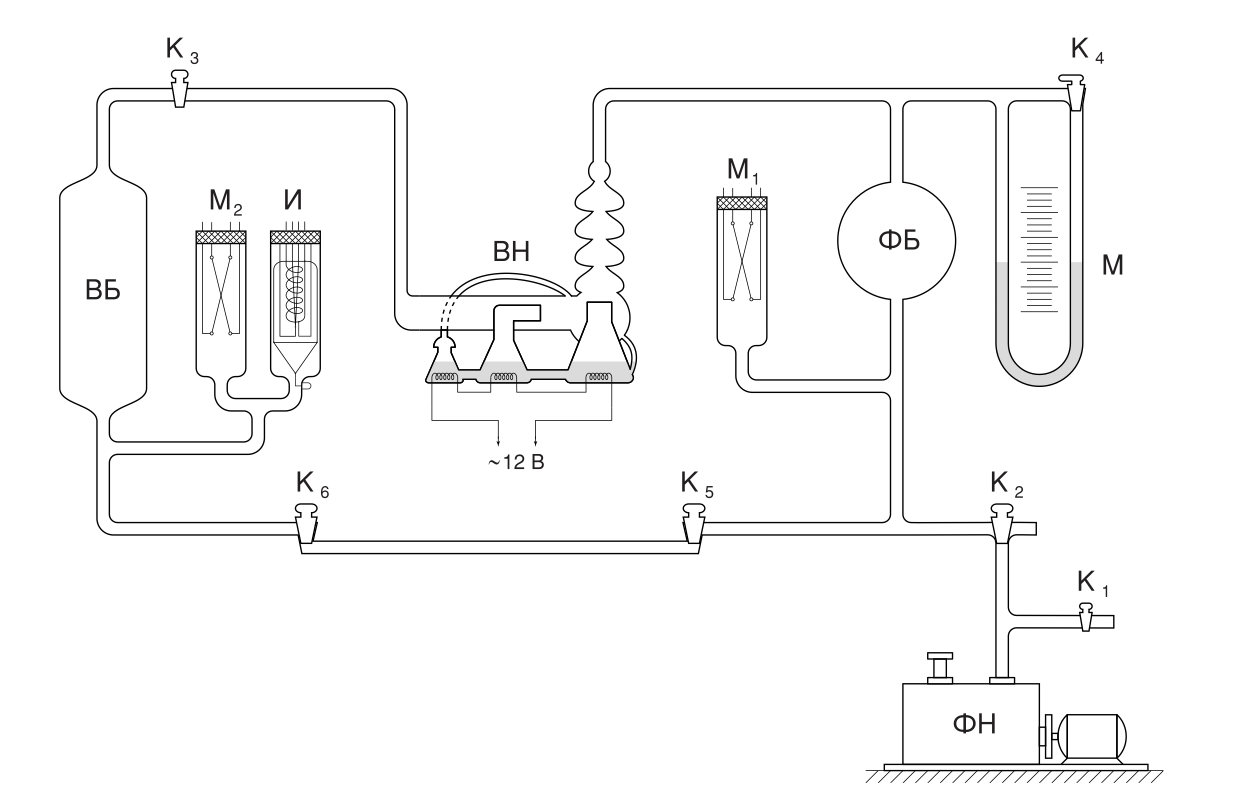
\includegraphics[width=\textwidth]{ust.png}}
		\caption{Схема установки}
	\end{figure}

    Установка изготовлена из стекла, и состоит из форвакуумного баллона (ФБ), высоковакуумного диффузионного насоса (ВН), высоковакуумного баллона (ВБ), масляного (М) и ионизационного (И) манометров, термопарных манометров (М1 и М2), форвакуумного насоса (ФН) и соединительных кранов (K1,K2, ... K6). Кроме того, в состав установки входят: реостат и амперметр для регулирования тока нагревателя диффузионного насоса.
	
    \subsection*{Методика измерений}
    \begin{enumerate}
    \item
	    Определим объемы форвакуумной и высоковакуумной частей установки. Сначала впустим атмосферу в установку. Запрем воздух при комнатных условиях в капилляре между кранами 5 и 6. После этого откачаем воздух из оставшейся части установки (сделав это в два этапа - сначала насос должен откачать сам себя, а только потом - установку). После этого мы сначала высвободим запертый воздух только в ФВ часть, а затем добавим к ней и ВВ. Тогда записав уравнение Менделеева-Клапейрона и зная объем капилляра, мы найдем объемы соответствующих частей установки:
    \begin{equation}
	    P_0 V_0 = P_v (V_f + V_v),
    \end{equation}
    где $P_0$ -- атмосферное давление; $V_0$ -- объем капилляра и кранов 5 и 6; $P_v$ -- установившееся давление; $V_f$ и $V_v$ -- соотвественно объемы форвауумной и высоковакуумной частей.
	
    \item
	    Для измерения скорости откачки диффузионного насоса измерим улучшение вакуума во времени. Построим график зависимости $-\ln{\frac{P-P_{pr}}{P_0}}$ от $t$. Из формулы(4) следует, что наклон, построенной кривой, есть $W / V$

    \item
	    Откроем кран 6 и создадим исскуственную течь через капилляр. Рассчитаем производительность насоса по различию $P_{pr}$ и $P_u$, где $P_u$ -- установившееся давление в высоковакуумной части с искусственной течью. В условиях высокого вакуума справдлива формула(6), где положим $P_1 := P_u$, $P_2$ -- давление в форвакуумной части. 
    \end{enumerate}

    \section{Результаты измерений и обработка данных}

    \subsection*{Определение объема форвакуумной и высоковакуумной частей установки}

    В таблице  приведены параметры установки.
	

    \begin{table}[H]
        \centering
    \begin{tabular}{|c|c|c|}
    \hline
    $\rho$, кг/м$^3$ & $V_0$, см$^3$ & $P_0$, торр  \\ \hline
     885              &     50        &    738                        \\ \hline
    \end{tabular}
    \caption{Некоторые параметры установки.}
    \end{table}

    \begin{table}[!ht]
        \centering
        \begin{tabular}{|c|c|c|c|c|c|c|c|c|}
        \hline
            $h_{1фор}$, см & $h_{2фор}$, см & $\Delta h_{фор}$, см  & $h_{1вместе}$, см  & $h_{2вместе}$, см & $\Delta h_{вместе}$, см & $V_{фор}$ & $V_{вместе}$ & $V_{выс}$ \\ \hline
            12 & 38,5 & 26,5 & 17 & 33,9 & 16,9 & 2139,8 & 3355,3 & 1215,5 \\ \hline
        \end{tabular}
        \caption{Таблица полученных объемов}
    \end{table}

    Чтобы найти объемы сосудов проведем измерения согласно описанию работы. По формуле Бойля Мариотта 
    \[ P_0 V_0 = p V_{сосуда} \]

    где $p$ считаем по формуле $\rho g \Delta h$ 

    \[ V = \dfrac{P_0 V_0}{\rho g \Delta h} \] 

    Сначала подставим $\Delta h$ для фор. части, найдем объем форвакуумной. Потом возьмем для обоих вместе и найдем обьедененный объем. 

    Относительная погрешность сосудов будет равна относительной погрешности $\Delta h$, поэтому
    
	\subsection*{Получение высокого вакуума и измерение скорости откачки}

    Открываем все краны и проводим первоначальную выкачку воздуха форвакуумным насосом. После приближения к предельному давлению ($\sim 10^{-2}торр$), закрываем кран 6 и включаем диффузионный насос. Ждем пока масло закипит и начнется дальнейшая выкачка уже диффузионным насосом. По достижению давления порядка $\sim 10^{-3}торр$ включаем ионизационный манометр, которым и будем измерять давление в дальнейшем.

    Чтобы измерить скорость откачки $W$ замерим как изменяется давление в высоковакуумной части от времени. Сосгласно теории давление должно падать по правилу, где у нас $P_{пр}=4,7\cdot10^{-5}торр$
    \begin{equation}
        P-P_{пр}=(P_0 - P_{пр})\exp\left(-\frac{W}{V_{вв}}t\right)
    \end{equation}
    Логарифмируя, получаем
    \begin{equation}
        \ln(P-P_{пр})=-\frac{W}{V_{вв}}t + c
    \end{equation}
    Аппроксимируя наши данные согласно формуле получим значение для $W$. Измерение проведем 2 раза. Результаты изображены на графиках.


    \begin{table}[!ht]
        \centering
        \begin{tabular}{|c|c|c|c|c|c|c|c|c|c|}
        \hline
            $t$, c & $P$ мм & $t$, c & $P$ мм & ln$(P-P_0)$ & $t$, c & $P$ мм &  $t$, c & $P$ мм & ln$(P-P_0)$ \\ \hline
            0 & 5,3 & 0 & 52 & 3,86 & 0 & 5,4 & 0 & 50 & 3,8 \\ \hline
            3 & 5,7 & 2 & 44 & 3,67 & 3 & 6,7 & 3 & 36 & 3,44 \\ \hline
            7 & 8,3 & 4 & 31 & 3,27 & 7 & 9,4 & 6 & 23 & 2,91 \\ \hline
            12 & 12 & 6 & 21 & 2,79 & 12 & 14 & 10 & 12 & 1,99 \\ \hline
            16 & 15 & 8 & 17 & 2,51 & 18 & 16 & 14 & 7,8 & 1,33 \\ \hline
            21 & 19 & 11 & 10 & 1,67 & 23 & 21 & 16 & 6,7 & 0,69 \\ \hline
            28 & 24 & 14 & 7,7 & 1,10 & 29 & 26 & 19 & 5,5 & -0,22 \\ \hline
            35 & 29 & 17 & 6,6 & 0,64 & 34 & 29 & 22 & 5,2 & -0,69 \\ \hline
            43 & 35 & 19 & 5,8 & 0,10 & 44 & 36 & ~ & ~ & ~ \\ \hline
            55 & 41 & 22 & 5,5 & -0,22 & 50 & 39 & ~ & ~ & ~ \\ \hline
            64 & 47 & 26 & 5,2 & -0,69 & 57 & 44 & ~ & ~ & ~ \\ \hline
            72 & 52 & ~ & ~ & ~ & 64 & 50 \\ \hline
        \end{tabular}
        \caption{Результаты измерений}
    \end{table}

    \begin{figure}[!ht]
		\center{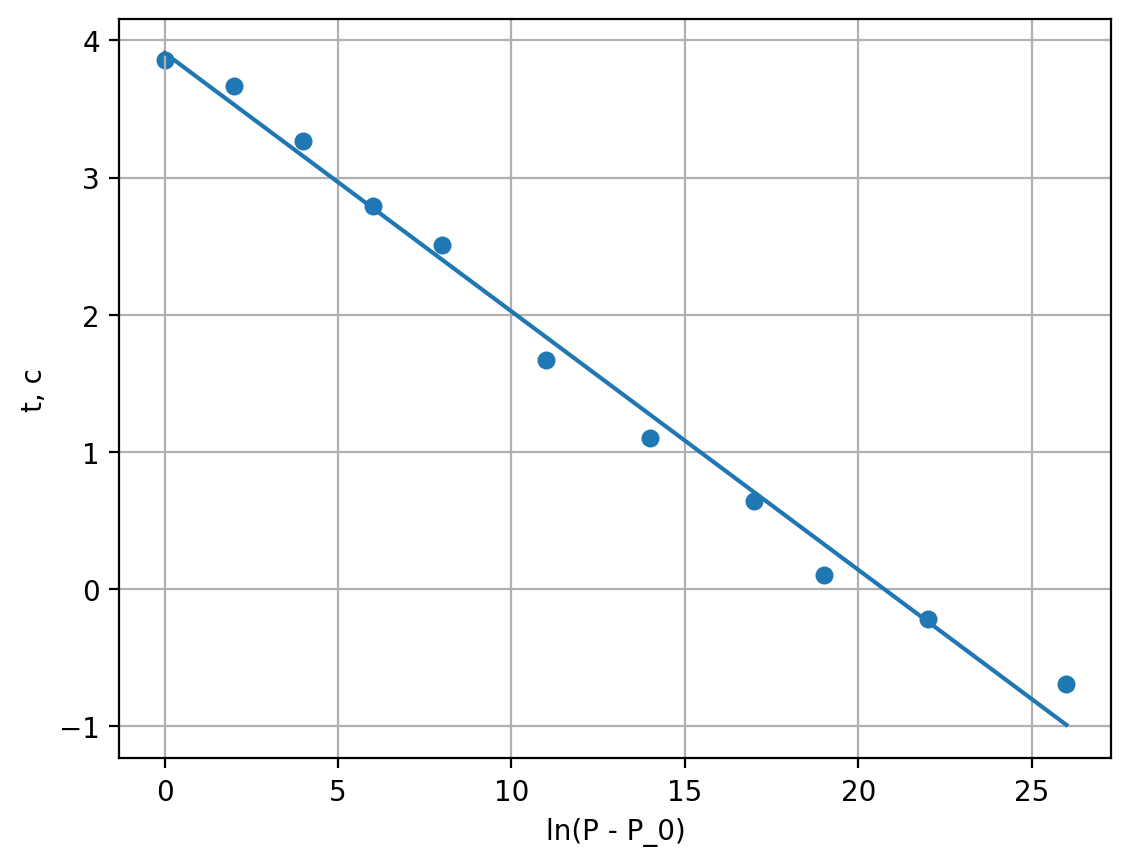
\includegraphics[width=0.7\textwidth]{first.png}}
		\caption{График для первого повышения}
	\end{figure}

    \begin{figure}[!ht]
		\center{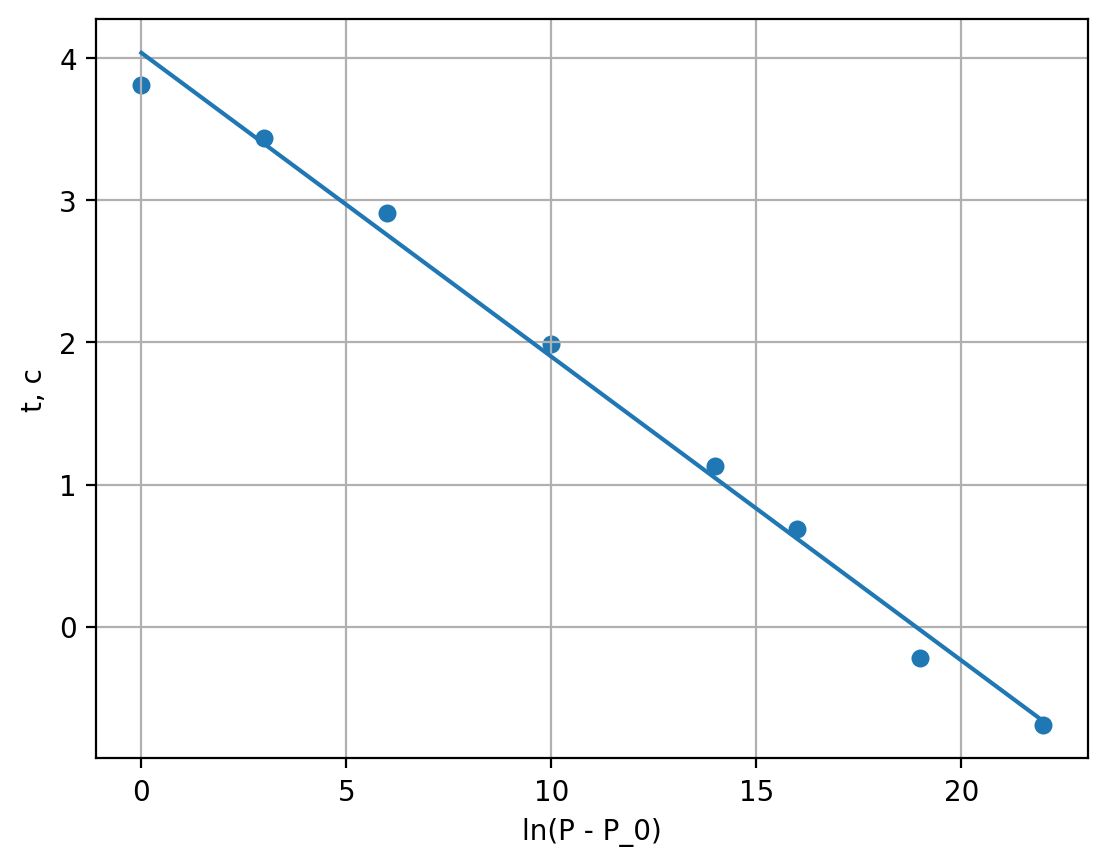
\includegraphics[width=0.7\textwidth]{second.png}}
		\caption{График для второго повышения}
	\end{figure}

    \[ k_1 = -(0.188 \pm 0.006) ~  с^{-1} \] 
    \[ k_2 = -(0.213 \pm 0.007) ~  с^{-1} \] 
    \[ k_{ср} = -(0.200 \pm 0.007) ~  с^{-1} \] 

    \begin{equation}
        W = (244 \pm 7)\frac{см^3}{с}
    \end{equation}

    Теперь определим величину потока $Q_н$. Для обшего потока имеем формулу
    \begin{equation}
        P_{пр}W = (Q_1 + Q_н)RT
    \end{equation}
    где $Q_1 = Q_и + Q_д$. Теперь, если по достижению предельного давления закрыть кран 3, то насос будет отсоиденен от высоковакуумной части, и уравнение описывающее давление от времени примет вид

    \begin{equation*}
        V_{вв}dP = Q_1 RTdt
    \end{equation*}
    интегрируя которую получим
    \begin{equation}
        P = \frac{Q_1 RT}{V_{вв}}t + c
    \end{equation}
    Измерив зависимость давления от времени и аппроксимируя данные прямой можно получить $Q$. Отсюда получаем
    
    \[ k_1 = (0.67 \pm 0.001) \cdot 10^{-5} \text{ } \dfrac{\text{ торр}}{с} \] 
    \[ k_2 = (0.7 \pm 0.001) \cdot 10^{-5} \text{ } \dfrac{\text{ торр}}{с} \] 
    \[ k_{ср} = (0.69 \pm 0.001) \cdot 10^{-5} \text{ } \dfrac{\text{ торр}}{с} \] 
    
    \begin{equation}
        Q_1 =(84 \pm 4)\cdot 10^{-4} ~ торр\cdot \text{ }см^3с^{-1}
    \end{equation}

    Используя формулу $Q_Н = P_{пр}W - Q_1$ получим, что: $Q_Н = (3,10 \pm 0.14) \cdot 10^{-3} ~ торр \cdot см^3 / с.$
		

    \begin{figure}[!ht]
		\center{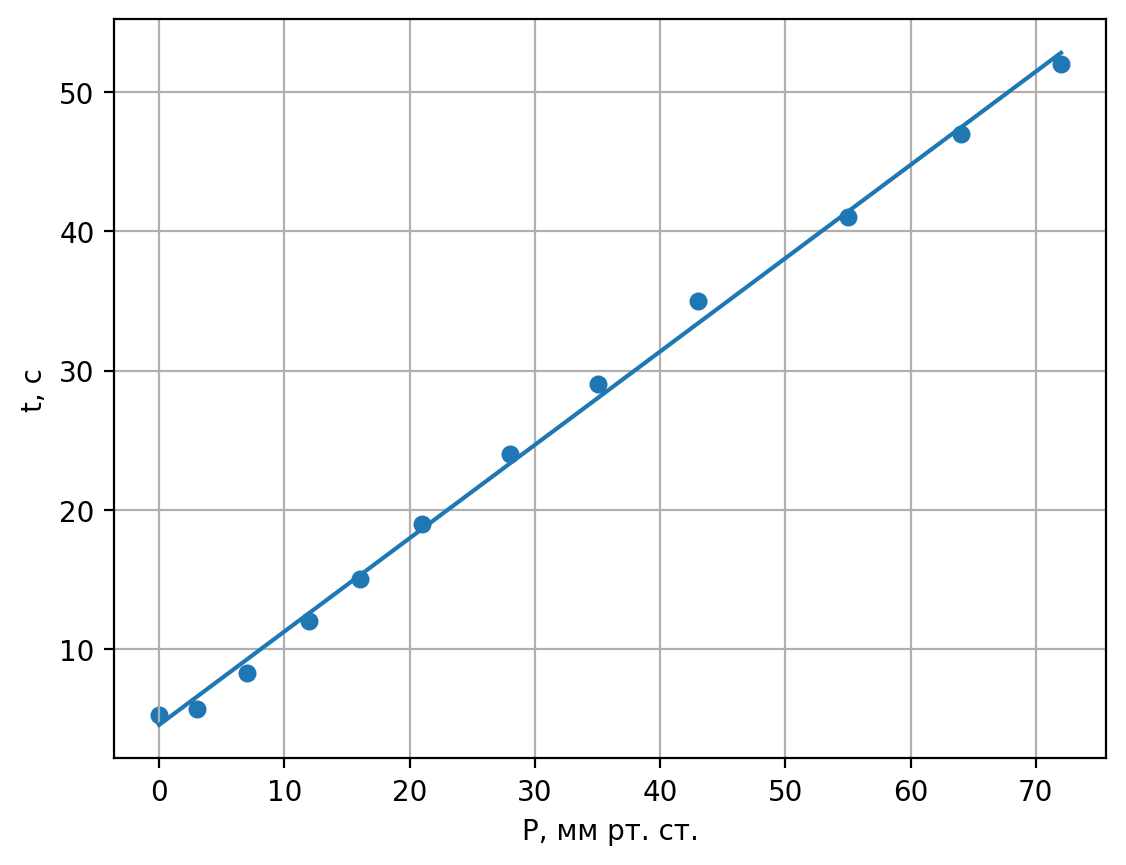
\includegraphics[width=0.7\textwidth]{third.png}}
		\caption{График для первого понижения}
	\end{figure}

    \begin{figure}[!ht]
		\center{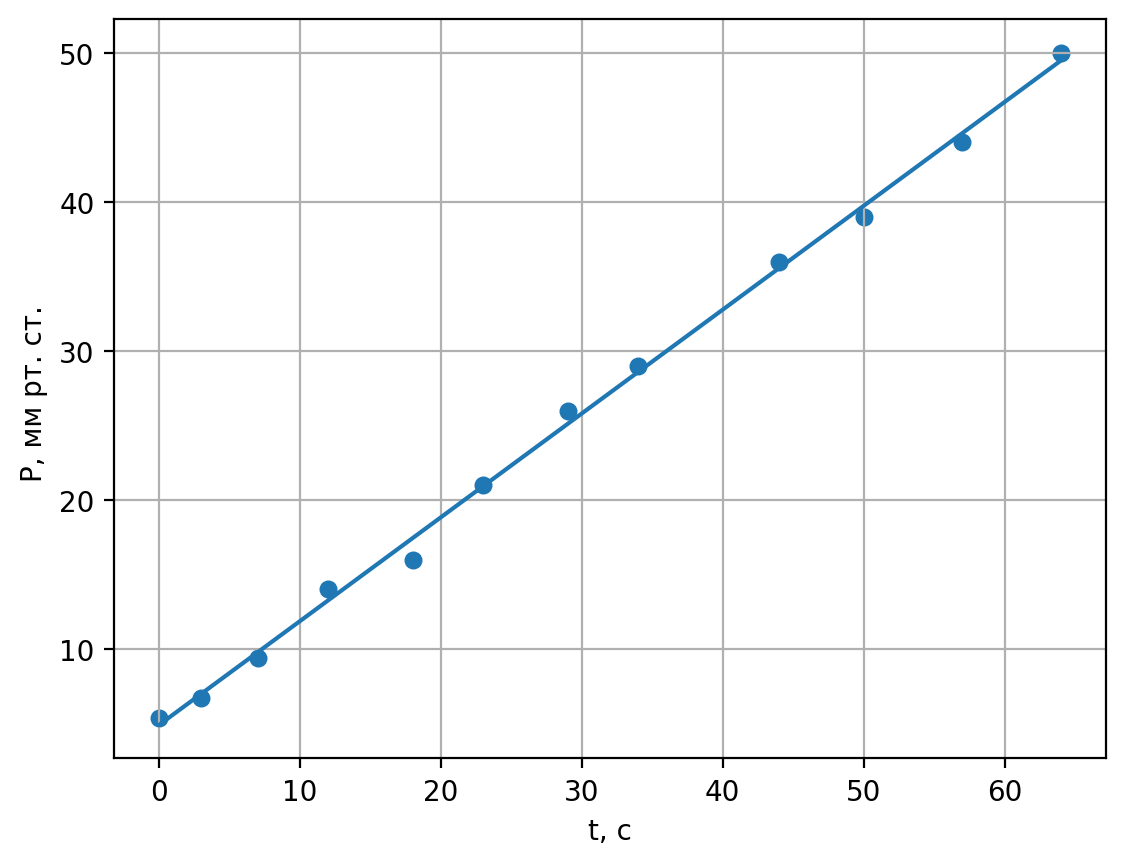
\includegraphics[width=0.7\textwidth]{four.png}}
		\caption{График для второго понижения}
	\end{figure}


    \newpage

    \subsection*{Измерение скорости откачки путем создания исскуственной течи}
    Открывая краны 5 и 6 мы создаем исскуственную течь через каппиляр. Измеряя изменение давления при создании течи можно посчитать производительность насоса. Опишем данную мысль математически. Обозначим $P_{вв}$ -- давление в высоковакуумной части, а $P_{фв}$ -- давление в форвакуумной части. До открытия каппиляра
    \begin{equation}
        \frac{P_{пр}W}{RT} = Q
    \end{equation}
    а после открытия
    \begin{equation}
        \frac{P_{уст}W}{RT} = Q + Q_{кап}
    \end{equation}
    где $P_{уст}$ -- установившееся давление после открытия капилляра, а $C_{тр}$ -- пропускная способность капилляра. В нашей установке

        Оценим пропускную способность трубки:
		\begin{align}
			L = (10.8 \pm 0.1)~ см; &&   d = (0.8 \pm 0.1) ~ мм,
		\end{align}
		
		\begin{equation}
			C_{тр} = (5.7 \pm 0.3) \cdot  10^{-7} ~ м^3 / с.
		\end{equation}



    \begin{align*}
        P_{пр}&=(4,7 \pm 0.1)\cdot10^{-5} \text{ торр}\\
        P_{уст}&=(8 \pm 0.1)\cdot10^{-5} \text{ торр}\\
        P_{фв}&=(4 \pm 0.1)\cdot 10^{-4} \text{ торр}\\
        T&=295 \text{ K}\\
    \end{align*}
    Подставляя числа получаем
    \begin{equation}
        W = \frac{P_{фв}}{P_{уст}-P_{пр}}\frac{4r^3}{3L}\sqrt{\frac{2\pi RT}{\mu}} \approx 7~\frac{см^3}{с}
    \end{equation}


    \section{Выводы}

    В данной лабораторной работе мы определили скорость откачки системы в стационарном режиме, а также по ухудшению и по улучшению вакуума. 
    Нашли объемы форвакуумной, высоковакуумной части установки. 
    Возможные расхождения данных могли возникнуть из за изменения температуры, созданное нагреваемым масляным высоковакуумным насосом. Возможно у манометра погрешность оказывала большое влияние на значение результатов, но из за того что мы ее не учитывали, получили разные данные. 
    Возможно, пропускная способность капилляра сильно занижает скорость откачки. 

    Вакуум в установке ухудшается и улучшается. Удалось линеаризовать эти зависимости.  в хорошем результате помогают убедиться графики, на которых прослеживается линейная зависимость (для улучшения вакуума -- линейная зависимость $\ln ((P-P_0) / (P_0 - P_{пр}))$ от $t$, а для ухудшения -- $P(t))$.  

\end{document}